\documentclass[usenames,dvipsnames,tikz]{standalone}
\usepackage{xcolor}
\colorlet{tBlue}{RoyalBlue!35!Cerulean}
\colorlet{tRed}{Red}
\usepackage{tikz}
\usepackage{standalone}
\begin{document}
	
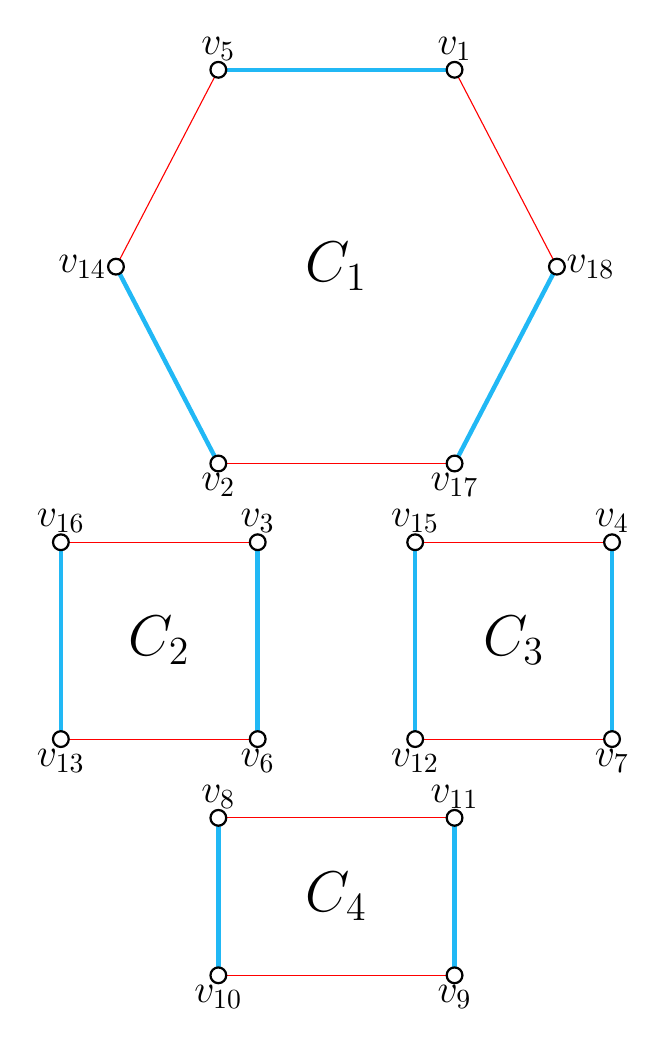
\begin{tikzpicture}
%v1=1, v2=1, v3=2, v4=2, v5=3, v6=4, v7=4, v8=5, v9=5, v10=6, v11=6, v12=6, v13=6, v14=7, v15=8, v16=9
%\draw [help lines] (-1,-1) grid (11, 15);

%C1 - blue
\draw [ultra thick, tBlue] (2,11.5) -- (5,11.5); 
\draw [ultra thick, tBlue] (2,6.5) -- (0.7,9); 
\draw [ultra thick, tBlue] (5,6.5) -- (6.3,9); 

%C2 - blue
\draw [ultra thick, tBlue] (0,3) -- (0,5.5); 
\draw [ultra thick, tBlue] (2.5,3) -- (2.5,5.5); 

%C3 - blue
\draw [ultra thick, tBlue] (4.5,3) -- (4.5,5.5); 
\draw [ultra thick, tBlue] (7,3) -- (7,5.5); 

%C4 - blue
\draw [ultra thick, tBlue] (2,0) -- (2,2); 
\draw [ultra thick, tBlue] (5,0) -- (5,2);

%C1 - red
\draw [tRed] (2,6.5) -- (5,6.5); 
\draw [tRed] (0.7,9) -- (2,11.5); 
\draw [tRed] (6.3,9) -- (5,11.5); 

%C2 - red
\draw [tRed] (0,3) -- (2.5,3); 
\draw [tRed] (0,5.5) -- (2.5,5.5); 

%C3 - red
\draw [tRed] (4.5,3) -- (7,3); 
\draw [tRed] (4.5,5.5) -- (7,5.5);

%C4 - red
\draw [tRed] (2,0) -- (5,0); 
\draw [tRed] (2,2) -- (5,2); 


%C1 - vertices
\draw [fill=white, thick] (2,6.5) circle [radius = 0.1]; %v2
\draw [fill=white, thick] (5,6.5) circle [radius = 0.1]; %v17
\draw [fill=white, thick] (0.7,9) circle [radius = 0.1]; %v14
\draw [fill=white, thick] (6.3,9) circle [radius = 0.1]; %v18
\draw [fill=white, thick] (2,11.5) circle [radius = 0.1]; %v5
\draw [fill=white, thick] (5,11.5) circle [radius = 0.1]; %v1

%C2 - vertices
\draw [fill=white, thick] (0,3) circle [radius = 0.1]; %v13
\draw [fill=white, thick] (2.5,3) circle [radius = 0.1]; %v6
\draw [fill=white, thick] (0,5.5) circle [radius = 0.1]; %v16
\draw [fill=white, thick] (2.5,5.5) circle [radius = 0.1]; %v3

%C3 - vertices
\draw [fill=white, thick] (4.5,3) circle [radius = 0.1]; %v12
\draw [fill=white, thick] (7,3) circle [radius = 0.1]; %v7
\draw [fill=white, thick] (4.5,5.5) circle [radius = 0.1]; %v15
\draw [fill=white, thick] (7,5.5) circle [radius = 0.1]; %v4

%C4 - vertices
\draw [fill=white, thick] (2,0) circle [radius = 0.1]; %v10
\draw [fill=white, thick] (5,0) circle [radius = 0.1]; %v5
\draw [fill=white, thick] (2,2) circle [radius = 0.1]; %v8
\draw [fill=white, thick] (5,2) circle [radius = 0.1]; %v11

%C1 - labels
\node [below] at (2,6.5) {\Large{$v_2$}};
\node [below] at (5,6.5) {\Large{$v_{17}$}};
\node [left] at (0.7,9) {\Large{$v_{14}$}};
\node [right] at (6.3,9) {\Large{$v_{18}$}};
\node [above] at (2,11.5) {\Large{$v_5$}};
\node [above] at (5,11.5) {\Large{$v_1$}};

%C2 - labels
\node [below] at (0,3) {\Large{$v_{13}$}};
\node [below] at (2.5,3) {\Large{$v_6$}};
\node [above] at (0,5.5) {\Large{$v_{16}$}};
\node [above] at (2.5,5.5) {\Large{$v_3$}};

%C3 - labels
\node [below] at (4.5,3) {\Large{$v_{12}$}};
\node [below] at (7,3) {\Large{$v_7$}};
\node [above] at (4.5,5.5) {\Large{$v_{15}$}};
\node [above] at (7,5.5) {\Large{$v_4$}};

%C4 - labels
\node [below] at (2,0) {\Large{$v_{10}$}};
\node [below] at (5,0) {\Large{$v_9$}};
\node [above] at (2,2) {\Large{$v_8$}};
\node [above] at (5,2) {\Large{$v_{11}$}};

%Component labels
\node at (3.5,9) {\huge{$C_1$}};
\node at (1.25,4.25) {\huge{$C_2$}};
\node at (5.75,4.25) {\huge{$C_3$}};
\node at (3.5,1) {\huge{$C_4$}};


\end{tikzpicture}
	
\end{document}
